
\begin{figure}[h]
\centering

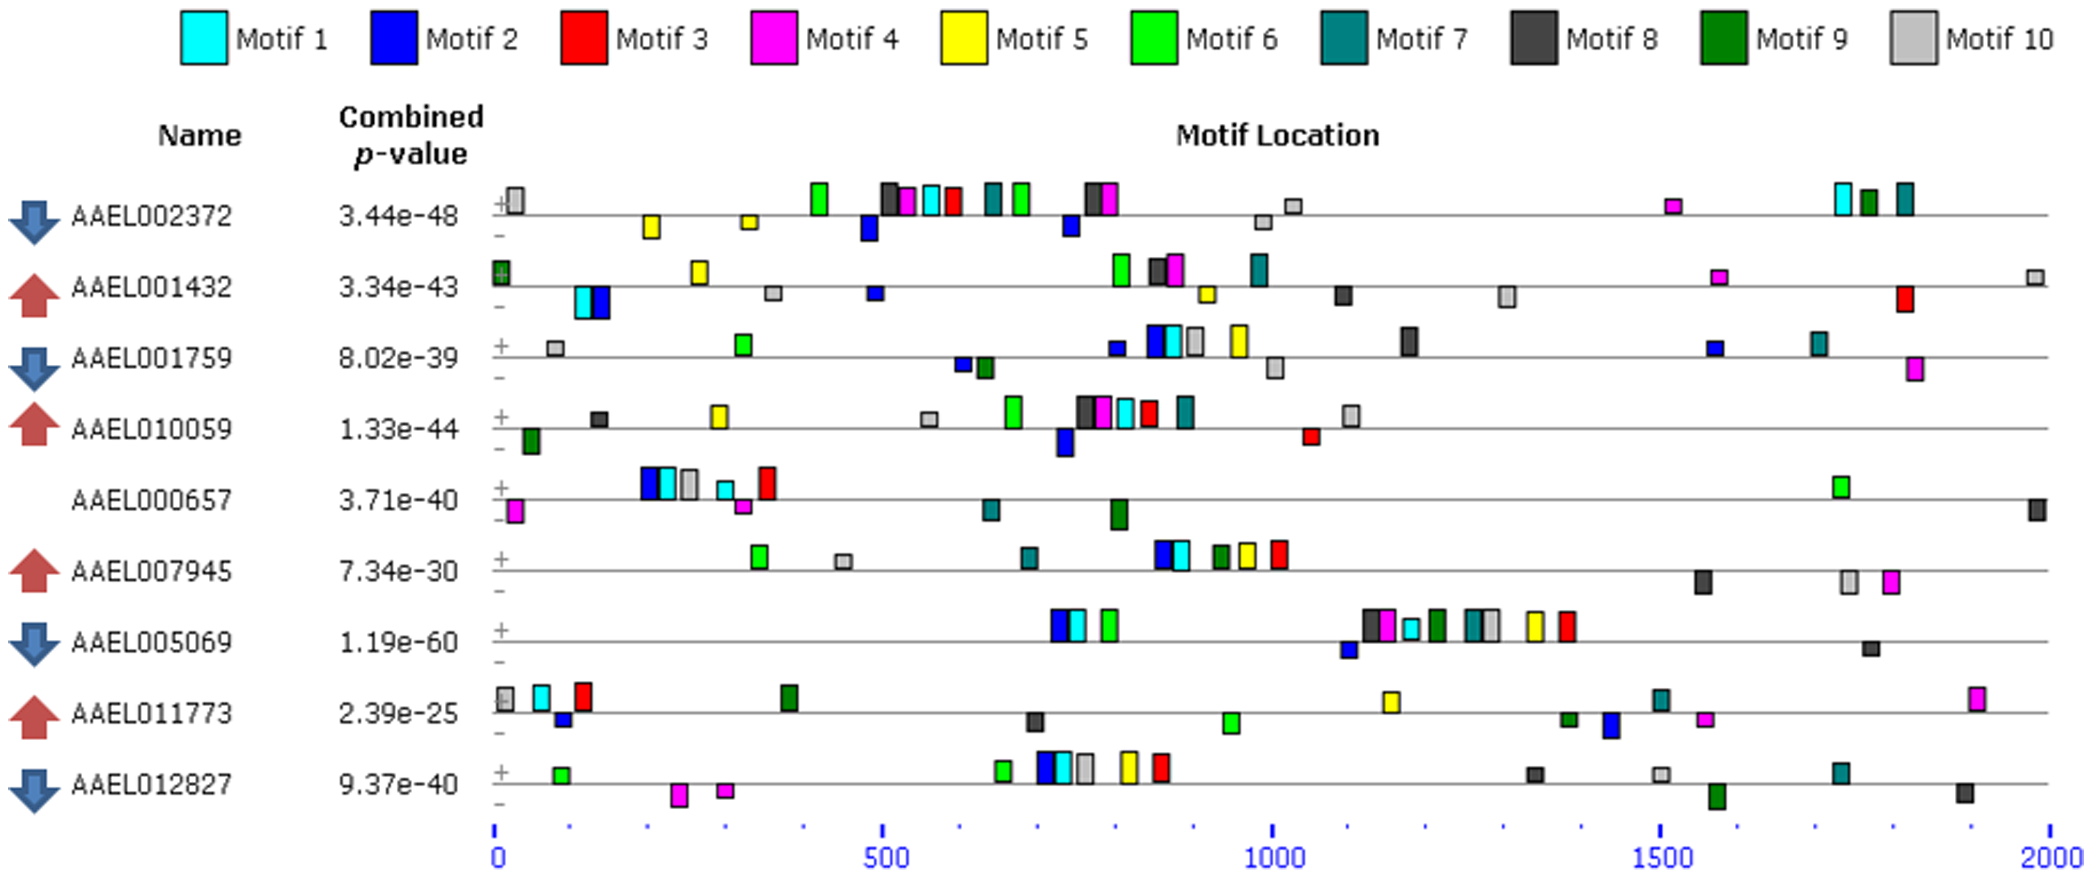
\includegraphics[width=.99\textwidth]{figures/figs/bonizzoni2012complex-cre.png}

\caption[MEME analysis of nine genes with \texorpdfstring{FPKM\textsubscript{DENVI}}{FPKM DENVI} ≥ 100 in carcasses and salivary glands at 14 dpi]{\sf \textbf{MEME analysis of nine genes with \texorpdfstring{FPKM\textsubscript{DENVI}}{FPKM DENVI} ≥ 100 in carcasses and salivary glands at 14 dpi} These genes also were identified with transcripts exhibiting significant differential accumulation in analyses of salivary gland samples of the Liverpool strain infected with DENV2 Thailand 16881 \cite{Luplertlop2011}. Colored boxes represent individual putative CREs and their locations in promoters of each gene. Red and blue arrows adjacent to Ensembl Gene ID indicate those genes whose transcripts were detected previously as more or less abundant following DENV infection \cite{Luplertlop2011}. Distances in base-pairs are provided below the schematic of each gene.
doi:10.1371/journal.pone.0050512.g004

Excerpted from \cite{bonizzoni2012complex}}
\label{fig:bonizzoni2012complex-cre}
\end{figure}

% \texorpdfstring{FPKM\textsubscript{DENVI}}{FPKM DENVI}